%
% File naaclhlt2016.tex
%

\documentclass[11pt,letterpaper]{article}
\usepackage{naaclhlt2016}
\usepackage{times}
\usepackage{latexsym}
\usepackage{graphicx}
\usepackage{subfigure} 
\usepackage{balance}
\usepackage{hyperref}
\usepackage{natbib}
\usepackage{arydshln}
\usepackage{enumitem}

\newcommand{\pred}{\bf}
%\newcommand{\pred}{\tt}
%\newcommand{\pred}{}
\newcommand{\squishlist}{
   \begin{list}{$\bullet$}
    { \setlength{\itemsep}{-1pt}      \setlength{\parsep}{3pt}
      \setlength{\topsep}{1pt}       \setlength{\partopsep}{0pt}
      \setlength{\leftmargin}{1.5em} \setlength{\labelwidth}{1em}
      \setlength{\labelsep}{0.5em} } }
\newcommand{\squishend}{
    \end{list}  }
    
\naaclfinalcopy % Uncomment this line for the final submission
\def\naaclpaperid{***} %  Enter the naacl Paper ID here
 
\newcommand\BibTeX{B{\sc ib}\TeX}

% \title{Machine Teaching for Information Extraction}
\title{IKE - A Machine Teaching Approach to Knowledge Extraction} 
% Love the User! Machine Teaching for Information Extraction

\author{Bhavana Dalvi\\
	    Allen Institute for \\ Artificial Intelligence\\
	    {\tt bhavanad@allenai.org}
	  \And
	Sumithra Bhakthavatsalam\\
  	Allen Institute for \\ Artificial Intelligence\\
	    {\tt sumithrab@allenai.org} 
  \And
	Peter Clark\\
  	Allen Institute for \\ Artificial Intelligence\\
	    {\tt peterc@allenai.org}}

\date{}

\begin{document}

\maketitle

\begin{abstract}
% Our long-term goal is a system that can answer sophisticated science questions, a task that seems to require reasoning over structured knowledge. This in turn requires an 
Any system that operates over structured knowledge needs an efficient and reliable way to acquire such knowledge, for example by extraction from text. Traditional information extraction research has focused on algorithms, and often requires long and complex iterations (often with a machine learning expert in the loop) to develop good extractors. In contrast, Machine Teaching focuses on the user, and how to most effectively leverage him/her to guide or ``teach'' the machine to perform a task well. Prior work suggests that a user is most effective when model updates are rapid, focused, and incremental, and that paying attention to this can dwarf minor algorithmic improvements in the learning algorithms themselves.
 
With this in mind, we have developed IKE, an interactive knowledge extraction tool that performs fast, interactive bootstrapping to develop high-quality extraction patterns for targeted relations. It allows quick exploration of the pattern space, and automatically suggests possible new patterns to explore based on relation mentions collected so far. A small, preliminary evaluation suggests that relation tables can be populated substantially faster than by manual pattern authoring or using fully automated tools, while retaining accuracy, an important step towards practical knowledge-base construction.

\end{abstract}

%-------------------------------------------------------

%\begin{figure*}[th]
%\begin{center}
%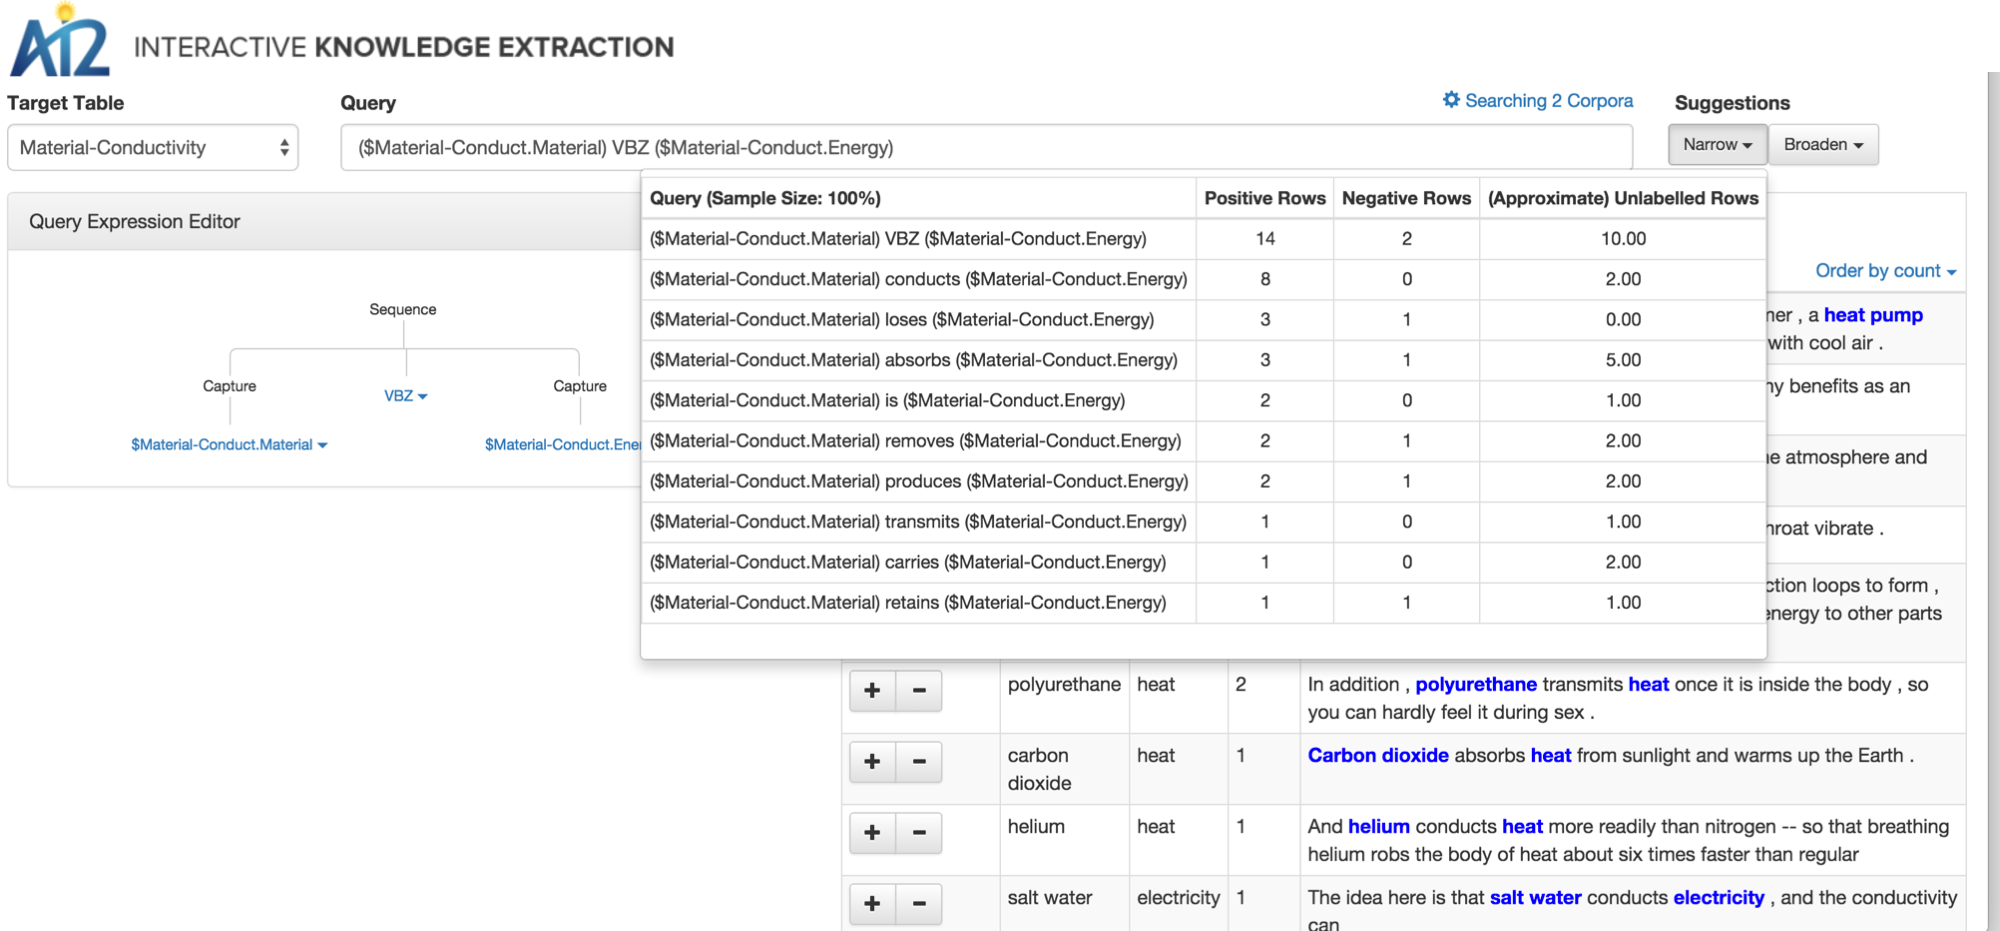
\includegraphics[scale =.5] {./figures/IKE_query_suggestions_narrow_2.pdf}
%\caption{Example of IKE query suggestions}
%\label{fig:IKE-query-suggest}
%\end{center}
%\end{figure*}

%\begin{figure}
%\includegraphics[width=\columnwidth]{./figures/conducts.png}
%\caption{Hi}
%\label{conducts}
%\end{figure}

\section{Introduction}

Knowledge extraction from text remains a fundamental challenge for any system that works with structured data. In our own project, Aristo, we are building a system to answer elementary science questions, and have found that many of these questions requires inference with structured knowledge \cite{clark:2016}. As a result, a key goal of ours is an efficient and reliable way to acquire structured knowledge from text.

Automatic information extraction algorithms (e.g., \cite{Angeli2015LeveragingLS}) have proved efficient, but typically produce noisy results (e.g., the best F1 score for the KBP slot filling task was 0.28, as reported in  \cite{Angeli2015LeveragingLS}). Weakly supervised automatic bootstrapping methods \cite{Carlson:wsdm2010,Gupta2014ImprovedPL} are more precise in the initial bootstrapping iterations, but digress in later iterations, a problem generally referred to as semantic drift. 
% In addition, these approaches have been limited to binary relation extraction.
 
More recently there has been work on more interactive methods, which can be seen as a ``Machine Teaching'' approach to KB construction \cite{Amershi2014PowerTT,Amershi2015ModelTrackerRP}. The premise here is that a focus on the user can produce improvements that dwarf those obtainable by minor changes to the learning algorithms themselves. For example, Soderland et al.~\cite{Soderland2013OpenIE} showed that users can be surprisingly effective at authoring and refining extraction rules for a slot filling task. Subsequently, Hoffmann et al.~\cite{Hoffmann2015ExtremeEO} built on this work to create an interactive extraction tool, InstaRead, allowing user-in-the-loop bootstrapping. Although restricted to binary relations, and requiring a user with linguistic expertise in the loop, these earlier techniques allowed fast population of binary relations from text.

In this paper, we take the Machine Teaching approach further and present IKE, a new tool for Interactive Knowledge Extraction via interactive bootstrapping. Our approach is novel in two ways: it allows us to extract n-ary relations, and it is targeted towards a domain expert in the topic of relations to be built, rather than a linguistic expert, e.g., in our context, a user who has elementary grade science knowledge. IKE takes care of all the linguistic processing including POS tagging, chunking, indexing and computing co-occurrence statistics of patterns from a large dataset. It supports fast, interactive bootstrapping and includes several novel features including a simple but rich pattern language, use of embedding-based similarity measures for extraction, support for N-ary relations, support for user-defined data types, and an easy-to-use interface. Although IKE is still early in its development, a preliminary evaluation suggests that relation tables can be populated substantially faster than by manual pattern authoring or using fully automated extraction tools, while retaining accuracy, an important step towards practical knowledge-base construction.

%-------------------------------------------------------
\begin{figure}[bth]
\begin{center}
%   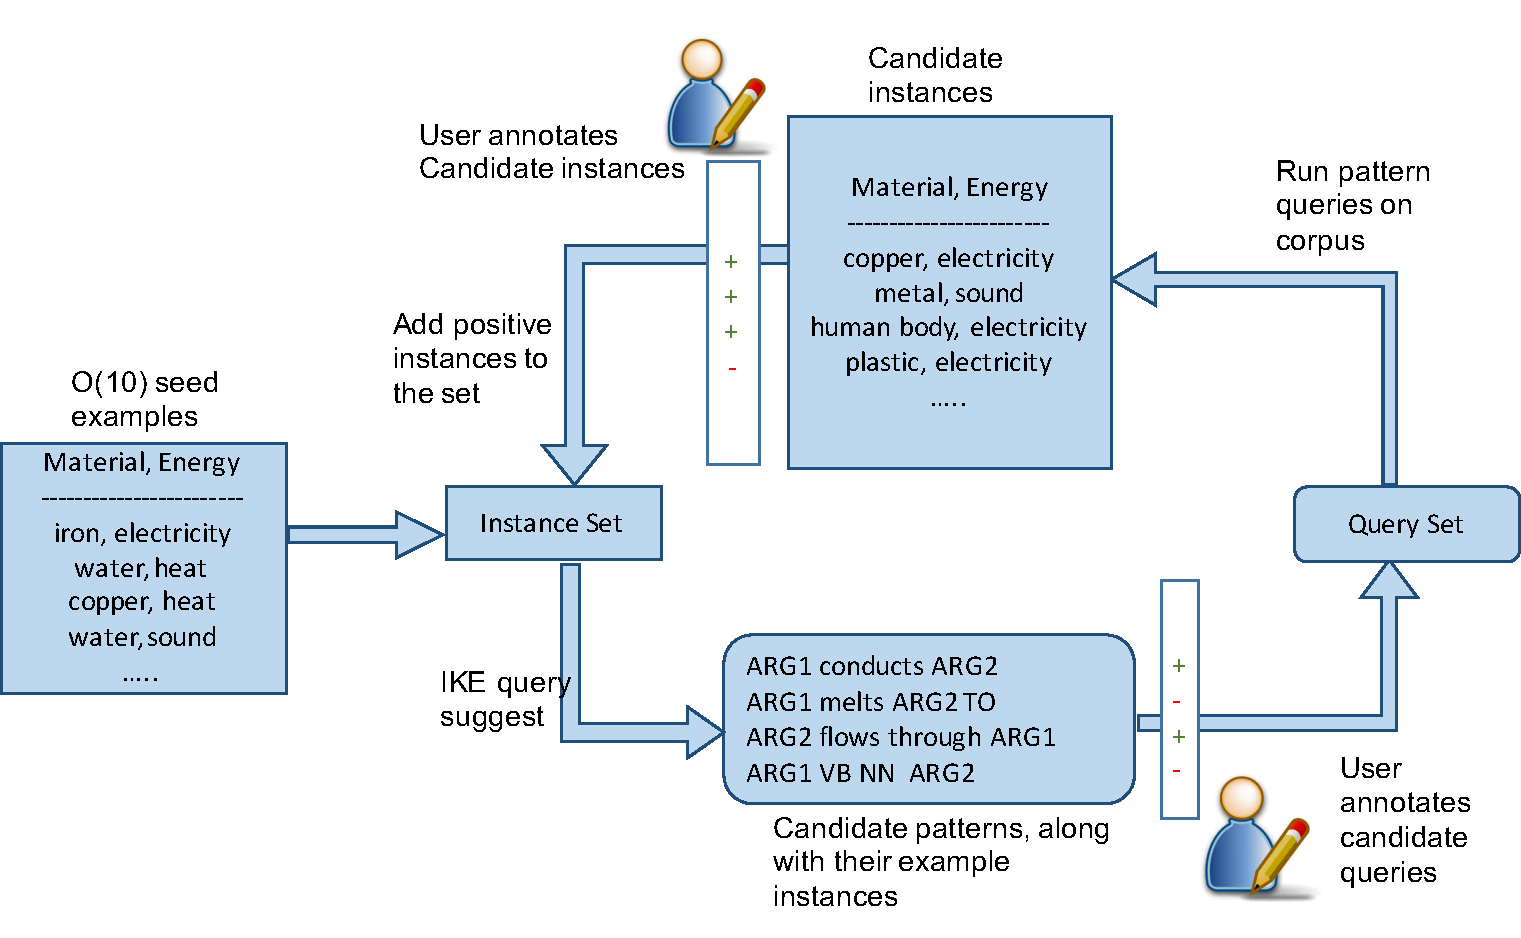
\includegraphics[scale =.25] {./figures/IKE_bootstrapping_ME_1.pdf}'
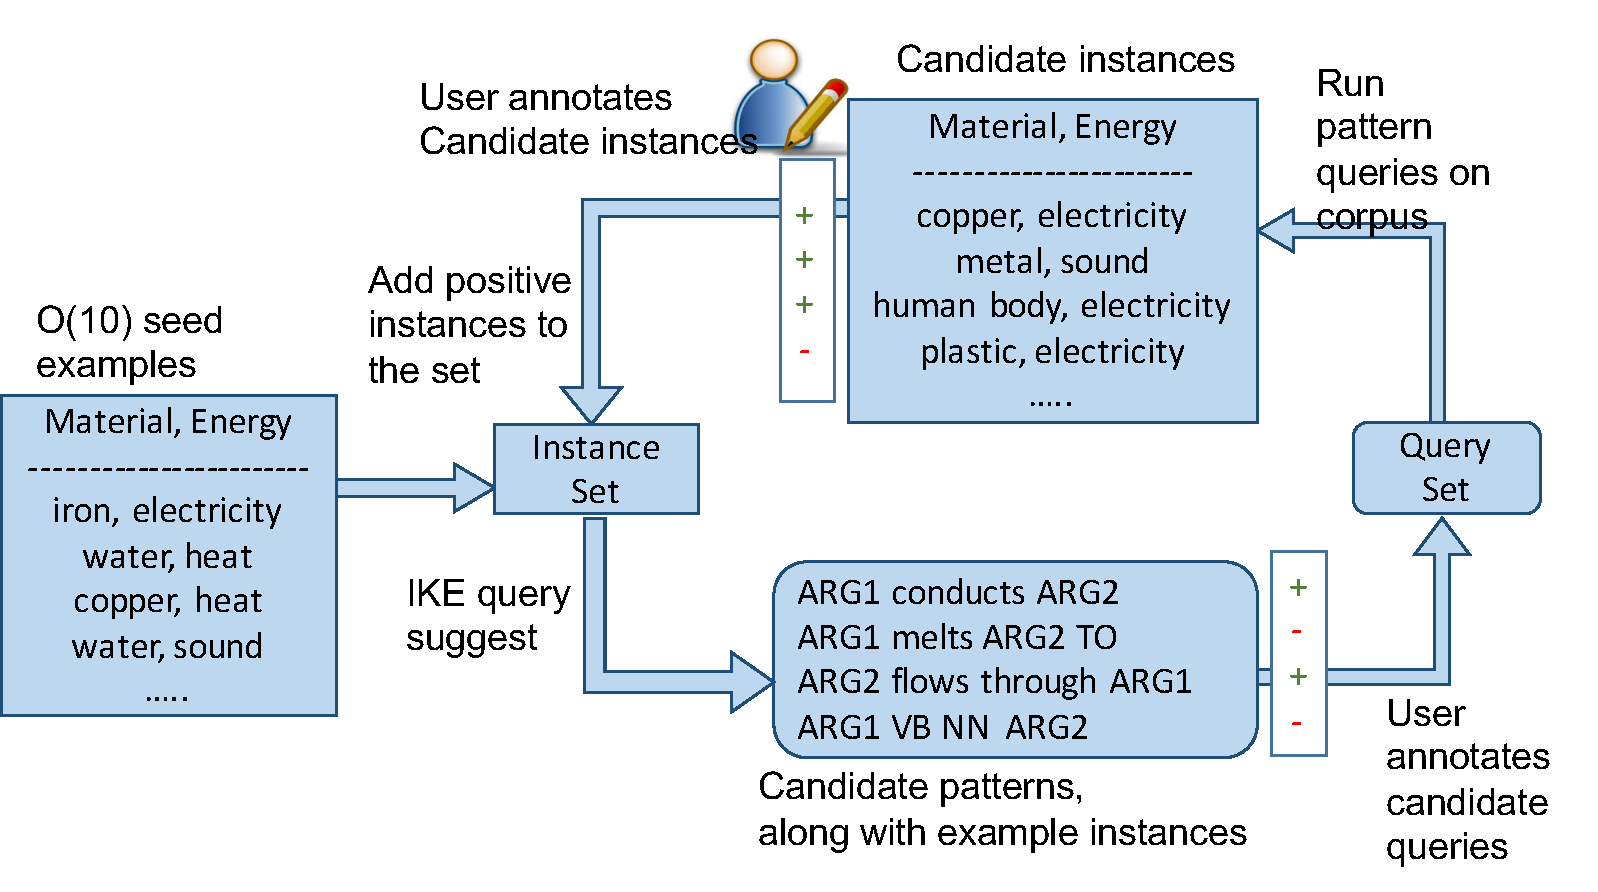
\includegraphics[width=\columnwidth] {./figures/IKE_bootstrapping_ME_3.pdf}
\caption{IKE interactive bootstrapping work-flow to create Material-Conductivity table}
\label{fig:IKE-Bootstrapping}
\end{center}
\end{figure}

\section{Interactive Knowledge Extraction (IKE)} \label{sect:IKE-description}

We first summarize the main features of IKE, and then provide more detail by describing a typical workflow to build a relation table. We will then present a preliminary evaluation of IKE in the subsequent Section.

\subsection{Overview}
IKE is a tool for relation extraction via interactive bootstrapping, with the following important features:
\squishlist
 \item pattern-based search over a corpus: extraction patterns are executable as search queries
 \item a rich query language: using regular expressions augmented with syntax for special IKE features (targets, reference to existing predicates, etc.).
 \item embedding-based set expansion: allowing vector-based similarity to be used in queries
 \item automatic query suggestion: using machine learning techniques
 \item support for use-defined entity types
 \item easy annotation of results
\squishend
Central to IKE is a search interface over the corpus. Users can issue regular expression queries that include ``capture groups'', indicated by parentheses. The results of these queries are the phrases that fill the capture groups, and each result populates a row in a table (i.e., the arguments of a predicate). For example, the query ``(NP) can conduct (NP)'' will find noun phrase pairs separated by ``can conduct'' in the corpus, and return those pairs. IKE uses BlackLab \cite{blacklab-tool} for indexing the corpus. This results in a rich query language supporting wildcards, window sizes, POS tags, chunk tags, as well as any existing IKE built knowledge tables. 

\subsection{IKE Query Language}

IKE uses Blacklab for indexing the corpus. This results in a rich query language supporting wildcards, window sizes, POS tags, chunk tags, as well as existing IKE built knowledge tables.
\begin{itemize}[noitemsep]
    \item Word sequences: A query ``the dog'' would match the word followed by the word ``cat''. 
    \item Part-of-speech (POS): A query ``DT dog'' would match a determiner a/an/the followed by the word ``dog''. IKE supports 36 POS symbols from the Penn Treebank \cite{Marcus1993BuildingAL}.
    \item Wildcards: The query ``. dog'' matches any word followed by the word "dog".
    \item Disjunctions: The query ``the \{cat$|$dog\}'' matches the word "the" followed by either "cat" or "dog". Similarly, a query ``the dog and the \{NN, NNS, NNP\}'' matches the phrase "the dog and the" followed by either a noun, a plural noun, or a proper noun.
    \item Repetitions: The query ``JJ* dog'' matches the word "dog" with zero or more adjectives before it. ``JJ+ dog'' matches the word "dog" with one or more adjectives before it, whereas a query ``JJ[2,4] dog'' would match the word "dog" with at least two but no more than four adjectives before it.
    \item capture groups: The query ``animals such as (?$<$Animal$>$ NN)'' captures a noun occurring after words ``animals such as'' and names the capture group as ``Animal''. Capture groups are used to fill entries in the target knowledge table.
    \item IKE built tables: IKE allows to refer to existing KB tables to be referred in the query. E.g. if there is an existing table {\pred has-part}({\it organism},{\it bodypart}), then a query can refer to organism column as ``\$has-part.organism''. 
    \item Similar words/phrases: IKE learns word2vec based embeddings of all words and popular phrases in a huge science corpus. These embeddings provide similarity distance between any two words/phrases, to enable searching for similar phrases. E.g. Query ``dog~50''	matches "dog" as well as the 50 words most similar to "dog". It also works with table queries. E.g. if there are 10 animals in the ``Animal'' table, then the query ``\$Animal ~100'' would find 100 phrases that are most similar to the items in the table.
\end{itemize}
    
\subsection{Example Workflow} \label{sect:IKE-workflow}

We now describe these features in more detail by way of an example. Consider the task of acquiring instances of the binary predicate {\pred conducts}({\it material},{\it energy}), e.g., conducts(``steel'',``electricity''). In IKE, relations are visualized as tables, so we treat this task as one of table population. The user's workflow can be summarized as follows:
\begin{enumerate}[noitemsep]
\item Define the types {\it material} and {\it energy}
\item Create a two-column table for {\pred conducts}
\item Use a seed pattern, e.g., ``X:{\it material} conducts Y:{\it energy}'', to populate the {\pred conducts} table with pairs (X,Y)
\item Repeat:
\begin{enumerate}[noitemsep]
  \item Use the ML-based query suggestor to find additional patterns relating the Xs and Ys, i.e., also expressing {\pred conducts}.
  \item Use those additional patterns to further populate {\pred conducts}
  \end{enumerate}
\end{enumerate}
This is the typical bootstrapping algorithm, here with a user in the loop. We now describe each of these steps.

\subsubsection{Define the types {\it material} and {\it energy}}

To define a type, IKE lets a user build a single column table. For example, to define the type {\it material}, the user:
\begin{enumerate}[noitemsep]
\item Creates a single column table called Material.
\item Manually adds several representative examples in the table, e.g., ``iron'', ``wood'', ``steel''.
\item Expands this set by searching for cosine-vector-similar phrases in the corpus, and marking valid and invalid members (Figure~\ref{material}). The syntax ``\$material $\sim$20'' denotes the 20 phrases most similar to any existing member in the {\it material} table, where similar is defined as the cosine vector between the phrase embeddings.
The parentheses ``()'' tells IKE that each result is a candidate new member for this table.
\item Repeat step 3 until the table adequately characterizes the intended notion of {\it material}
\end{enumerate}
The process is repeated for the type Energy.

\begin{figure}
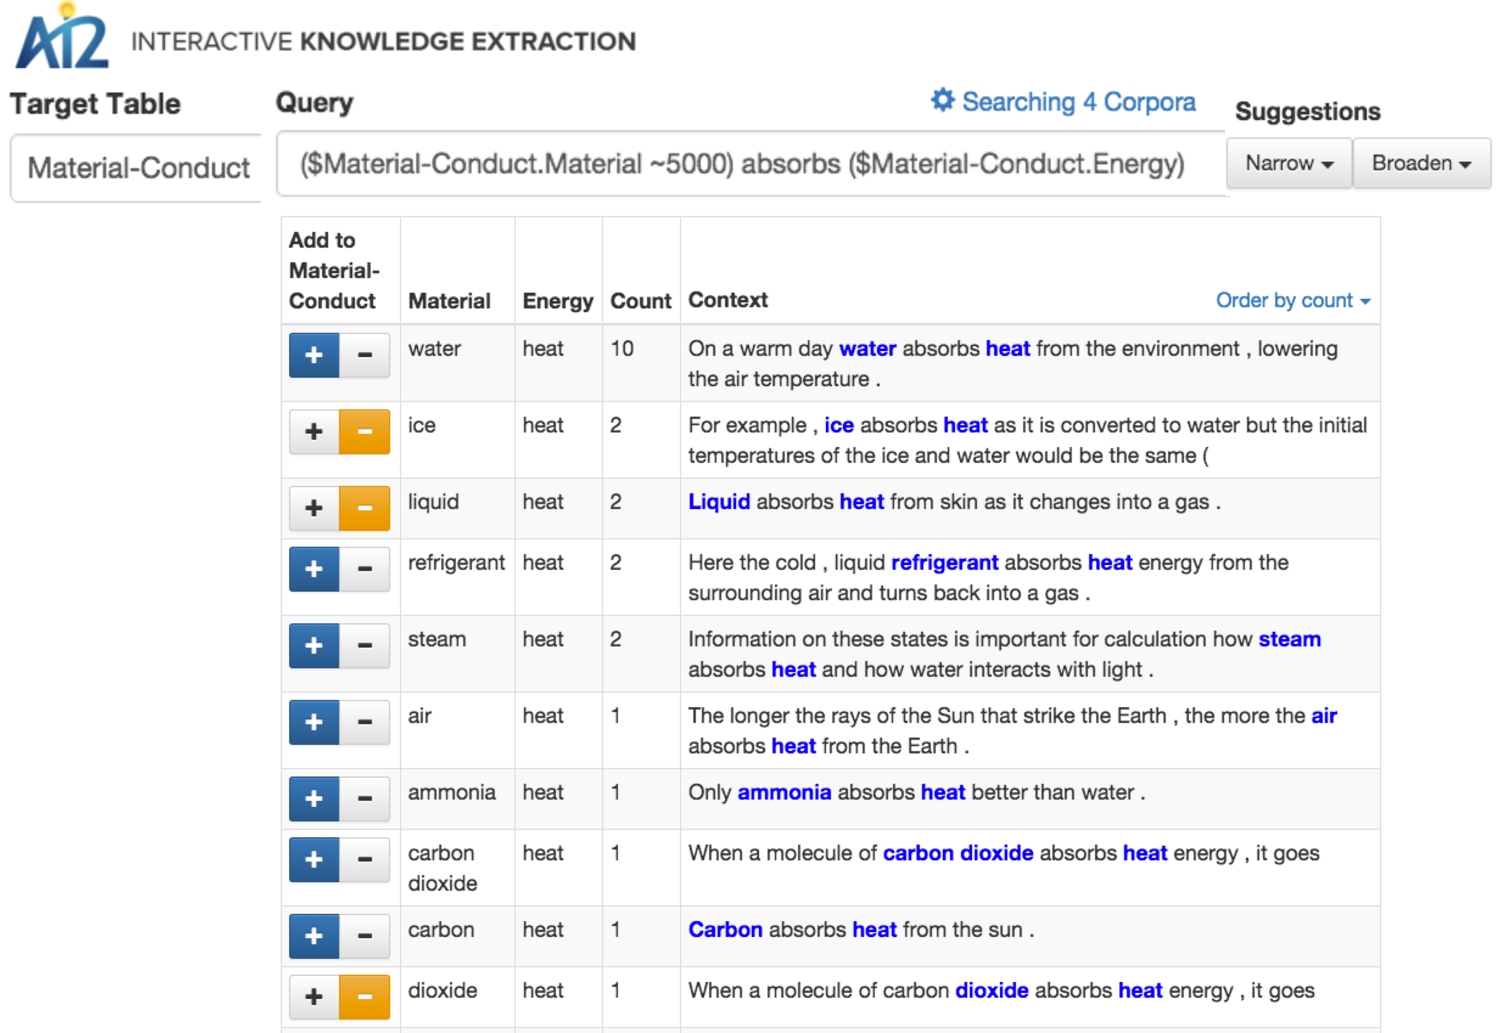
\includegraphics[width=\columnwidth]{./figures/IKE_relation_learning_2.pdf}
\caption{Use of set expansion to find and select vector-similar phrases in the corpus.}
\label{material}
\end{figure}

\subsubsection{Creation and Initial Population of {\pred conducts}}

The user next creates a two-column table {\pred conducts}, and then uses a seed pattern to find initial pairs to populate it, e.g., the pattern
\begin{quote}
``(\$Material) conducts (\$Energy)''
\end{quote}
extracts pairs of materials and energies they conduct. The user selects valid pairs to initially populate the table. Invalid pairs (negative examples) are also recorded by IKE.

\subsubsection{Bootstrapping to Expand the Table}

\begin{figure}
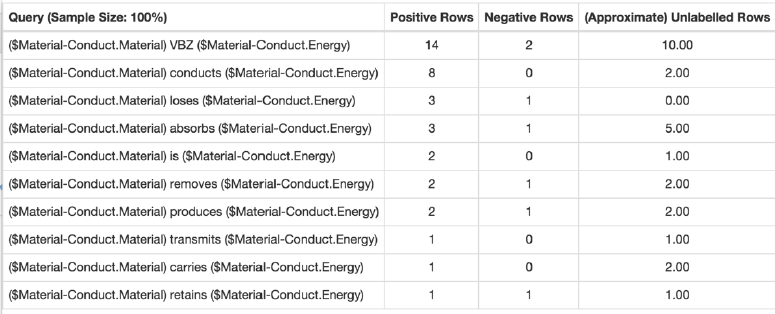
\includegraphics[width=\columnwidth]{./figures/query-suggestor.png}
\caption{IKE's Query Suggestor proposes additional patterns for the {\pred conducts} relation.}
\label{query-suggestor}
\end{figure}

The user can now bootstrap by invoking the Query Suggestor to find additional patterns (queries) that express the target relation, illustrated in Figure~\ref{query-suggestor}. It does so by searching for narrowings or broadenings of the current query that cover a large number of positive pairs and few negative pairs in the table so far. The user then clicks on one these patterns to select and execute it (possibly with edits if desired) to find more instances of the relation, mark good/bad pairs, and expand the table. This process can then be repeated.

Narrowing involves searching the space of restrictions on the current query, e.g., replacing a POS tag with a specific word, whereas the broaden feature generalizes the given user query e.g. replacing a word by its POS tag. In both cases the candidate queries are ranked based on the number of positive, negative, and unlabeled instances it produces. Figure \ref{query-suggestor} shows an example of narrowing a query for the {\pred conducts} table, where IKE has suggested several verbs found in the corpus, ranked by their ability to distinguish known positives from negatives in the table.
Although the suggested queries can sometimes look complicated with POS and chunk tags within them, the user only has to understand them, not author them from scratch. Hence the required skill set and data analysis workload on user is significantly reduced. The system still gives control to the user by letting him/her filter/edit the queries, and annotate the extractions in each iteration. 

By repeating this process, the user rapidly populates the table with positive examples. Negative examples are also recorded by IKE for use by the Query Suggestor.

\section{Experimental Evaluation} \label{sect:expt-eval}

\subsection{Experiments}

Although IKE is still under development, we have conducted a small, preliminary evaluation, comparing it with two other methods for populating relation tables. Our interest is in how these different methods compare in terms of precision, yield and time. The methods compared were:
\squishlist
\item \emph{Manual}: The user manually authors and refines patterns (without any automatic assistance) to populate a table.
\item \emph{Automatic}: The user provides an initial table with a few entries, and then lets the system bootstrap on its own, without any further interaction.
\item \emph{Interactive (IKE)}: Interactive bootstrapping, as described earlier.
\squishend
The manual system was implemented in IKE by disabling the embedding-based set expansion and query suggestion features. The automatic approach was simulated in IKE by removing both user annotation steps in Figure \ref{sect:IKE-workflow}, and instead adding all patterns and instances that occur at least $k$ times in the corpus (using $k$ = 2).

\subsection{Tasks and Datasets}

We compared these methods to define and populate two target relations: {\pred has-part}({\it animal},{\it bodypart}), and {\pred conducts}({\it material},{\it energy}).
% {\pred pollution}({\it source}, {\it pollutant}).
All methods extract knowledge from the same corpora of science text, consisting of $\sim$1.5M sentences (largely) about elementary science drawn from science textbooks, Simple Wikipedia, and the Web. For each relation, two (different) users familiar with IKE were asked to construct these tables. Although this study is small and preliminary, it provides some helpful indicators about the IKE's usefulness.

% make use of following four science text corpora (\#sentences in the parenthesis): Barron's study-guide for 4th grade science (1.2K), CK-12 corpora (17K), Simple Wikipedia ($\sim$1M), and Science subset of Waterloo corpus ($\sim$1.5M) \cite{waterloo-corpus}.

\subsection{Results}

\begin{table}[tbh]
\centering
\boldmath
\scalebox{0.75}{%
 \begin{tabular}{|l|cc|cc|c|} \hline
Method & \multicolumn{2}{|c|}{Acquired Patterns} & \multicolumn{2}{|c|}{Extractions} & Time \\
\cline{2-5}
 & No. of & Average & Number & Yield & in min.\\
 & patterns & Precision & (total) & (+ves) & \\ \hline
\emph{Manual}           &   5 & 66.7 &  24 & 16  & 30 \\
\emph{Automatic}        & 108 & 34.4 & 183 & 63 & -  \\ % \hdashline
\emph{IKE} &  41 & 59.2 & 142 & {\bf 84} & 20 \\ \hline
\end{tabular}
}
\caption{{\pred conducts}({\it material},{\it energy}) table: IKE helps the user discover substantially more patterns than the manual method (41 vs. 5), with similar precision and in less time, resulting in the overall highest yield. Fully automatic bootstrapping produced a large number of low precision patterns and overall lower yield than IKE.} 
\label{table:conducts}
\end{table}

\begin{table*}[tbh]
\centering
\boldmath
\scalebox{0.75}{%
 \begin{tabular}{|l|cc|cc|cc|} \hline
Method & \multicolumn{2}{|c|}{Acquired Patterns} & \multicolumn{2}{|c|}{Extractions} & \multicolumn{2}{|c|}{Time} \\
 \cline{2-5}
 & No. of & Average & Number & Yield & User time &Avg. query time\\
 & patterns & Precision & (total) & (+ves) & in min. & in sec. (\#queries)\\ \hline
\emph{Manual}           & 11 & 21.0 &  291 & 61 & 40 & 1.23 (35) \\
\emph{Automatic}        & 228 & 3.4 & 1386 & 48 & - & 2.6 (25) \\ % \hdashline
% \emph{Interactive (IKE)} & 21 & 57.4 & 249  & 143 &  30 \\ \hline
\emph{IKE} & 21 & 57.4 & 249  & {\bf 143} &  30 & 3.17 (24) \\ \hline
\end{tabular}
}
\caption{{\pred has-part}({\it organism},{\it bodypart}) table: Again, IKE produces the highest yield by helping the user discover substantially more (21) high-precision (57.4\%) patterns.}
\label{table:body-parts}
\end{table*}

Table \ref{table:conducts} shows the results for building the {\pred conducts}({\it material},{\it energy})table. Most importantly, with IKE the user was able to discover substantially more patterns (41 vs. 5) with similar accuracy (59.2\% vs. 66.7\%) than the manual approach, resulting in a larger table (84 vs. 16 rows) in less time (20 vs. 30 mins). It also shows that fully automatic bootstrapping produced a large number of low quality (34.4\% precision) rules, with an overall lower yield (63 rows). 
Table~\ref{table:body-parts} shows similar results for constructing the {\pred has-part}({\it organism},{\it bodypart}) table, again IKE having the highest overall yield.
Although this is a small study, it suggests that IKE has value for rapid knowledge base construction.

\begin{table*}[tbh]
\centering
\boldmath
\scalebox{0.75}{%
 \begin{tabular}{|l|c|c|} \hline
Corpus & \# sentences & Avg. query-time (sec.) \\
\hline
Barrons & 1.2K & 0.2533	\\ 
CK12 & 17K   & 0.2862	\\ 
SimpleWikipedia & 1M & 0.5296	\\
WaterlooFiltered (high-confidence) & 1.5M & 0.5953	\\ 
WaterlooFiltered & 20M & 2.809 \\
\hline
\end{tabular}
}
\caption{Avg. query-times with different sized corpora.}
\label{table:query-times}
\end{table*}

% **** \textbf{an example of n-ary relation with general phrases (Animal, Adaptation, Challenge), where adaptation is ``ADJ BODYPART''}

%-------------------------------------------------------

\subsection{Future Development}

IKE is still under development, with several areas needing further investigation. ...  {\bf elaborate}

% Currently IKE is trying to learn best extraction patterns for a target relation using manual annotations of instances and patterns. There is a possibility of improvement in the sense that the query suggestions for a relation can be based on a model for both arguments along with context between and around them. 
%-------------------------------------------------------
%\newpage
%\clearpage

% \section{Conclusions}  \label{sect:conclusions}

\section{Conclusion}

We have presented IKE, a tool that performs fast, interactive bootstrapping to develop high quality extraction patterns for targeted relations. It is an example of a Machine Teaching approach to knowledge base construction, where the focus is on leveraging the user to rapidly guide the system to good results. The preliminary evaluation comparing with manual and automated approaches, although small, is encouraging as it suggests that IKE makes the best of worlds by improving recall compared with a manual process while retaining precision within acceptable bounds. We are currently using IKE to expand the collection of tables used by the Aristo system \cite{clark:2016}.

%-----------------------------

\subsubsection*{Acknowledgments:} 
We also thank Tony Fader, Dirk Groeneveld, Oren Etzioni, and Chris Clark for their critical contributions to IKE.

%\clearpage
%\newpage
\bibliography{references}
\bibliographystyle{abbrv}

\end{document}
